\section{Experimental Methods and Time Series Explanations}\label{sec:methods}
{\color{blue} EDITABLE}
% \begin{enumerate}
% \item \cmark  Experimental methods: (how we collect the %time series and what the times series areThis should be HPM %PAPI, which programs we model
%\item \cmark program descriptions and relevant citations
%\subitem \cmark description of \col
%\subitem \cmark description of \gcc
%\subitem \cmark description of \svd 
%\subitem \cmark description of svd regimes
% \end{enumerate}


\subsection{Time Series Collection {\color{blue} EDITABLE}}

The time-series data for these experiments was collected on an Intel
Core\textsuperscript{\textregistered} i7-2600-based machine running
the 2.6.38-8 Linux kernel.  This particular microprocessor chip has
eight processing units---''cores''---a clock rate of 3.40GHz, and a
cache size of 8192 KB.  We collected performance traces of processor
efficiency during the execution of three different programs---the
simple loop (\col) whose performance is depicted in
Figure~\ref{fig:col-ipc} and two more-complex programs: one from the
SPEC 2006CPU benchmark suite (\gcc), and one from the LAPACK linear
algebra package (\svd).  To record these measurements, we used the
{\tt libpfm4} library, via PAPI
% 
% \footnote{Performance Application Programming Interface}
% 
5.2~\cite{papi}, to stop program execution at 100,000-instruction
intervals and read the contents of the CPU's onboard hardware
performance monitors\footnote{These specialty registers are built into
  modern microprocessors for the purpose of on-board monitoring and
  storage of performance data.}, which we had programmed to count how
many instructions were executed in each clock cycle (IPC).  For an
in-depth description of this custom-measurement infrastructure,
including discussion of the implications of the measurement interval,
please see \cite{zach-IDA10,mytkowicz09,todd-phd}.  For statistical
validation, we collected 15 performance traces from each of the three
programs.

% Obviously using a system to measure itself can cause
% interference--i.e, are you measuring the generating process cleanly or
% are you adding noise to the process?---but due diligence was put into
% monitoring the generating process of these time series without
% interfering with it in a significant way.


\subsection{The Programs: [[Maybe The generating processes]]{\color{blue} EDITABLE}}
We collect performance traces of processor efficiency (IPC) of three exemplar programs, [[If we change the title of the section, add this: which act as our generating processes]]---a simple microkernel(\col) and two complex programs: one from the
SPEC 2006CPU benchmark suite (\gcc), and one from LAPACK (\svd). In this section we provide a quick explanation of each program as well as an example performance trace (Seen in Figures \ref{fig:col-ts}-\ref{fig:svd-ts-colored}.
\subsubsection{\col {\color{blue} EDITABLE}}
\col is a simple three-line C program that repeatedly initializes the upper triangle of a  2048 X 2048 matrix in column-major order. While this is a very simple program it has been shown to produce time series with very complicated behavior. In fact, in \cite{mytkowicz09} it was shown that time series generated from this simple program can exhibit everything from periodicity to deterministic chaos.  A time series of the processor efficiency (IPC) of this program is shown in Figure \ref{fig:col-ts}.

\begin{figure}[htbp]
  \centering
    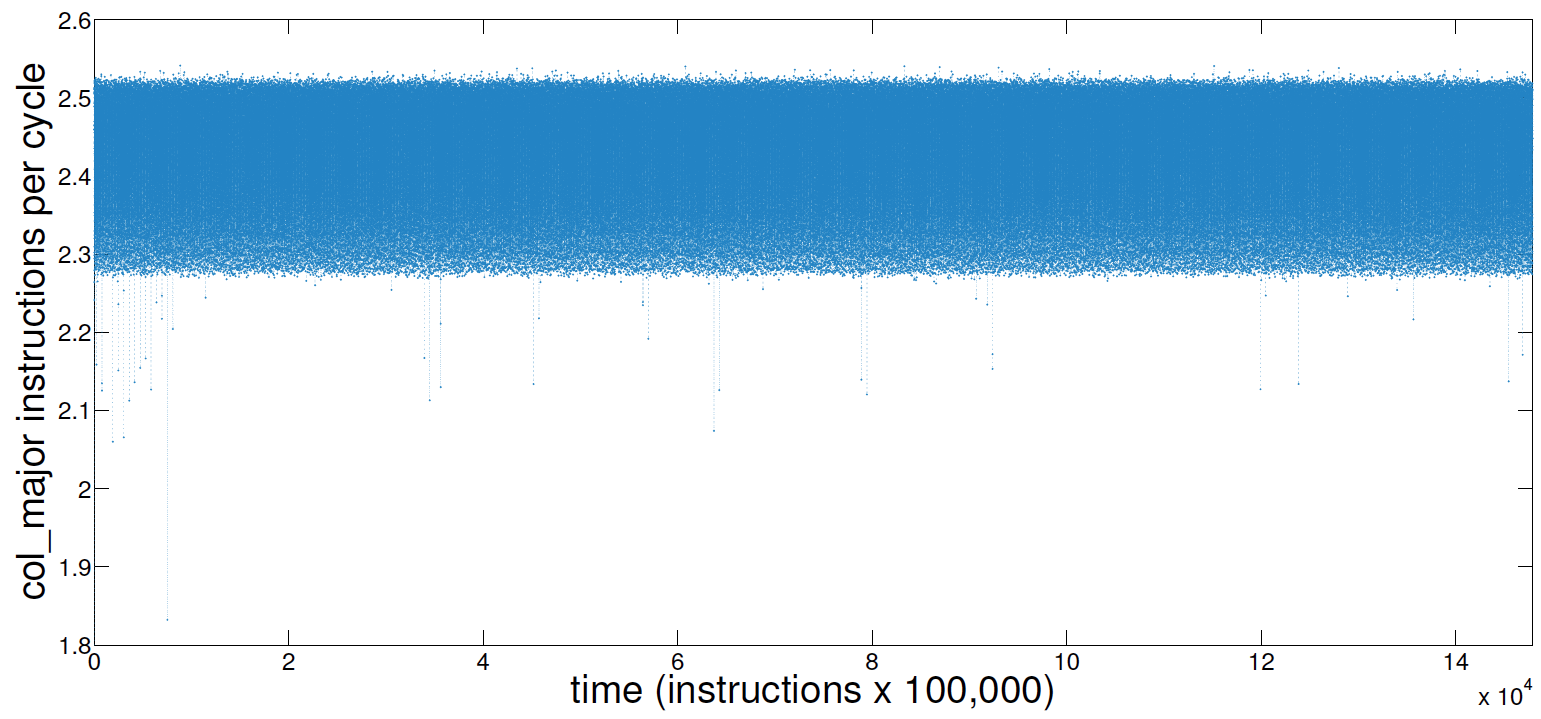
\includegraphics[width=\columnwidth]{figs/colFullTS}
    \caption{The instructions executed per CPU clock cycle (IPC) during the execution of \col. Each point is the average IPC during a 100,000 instruction period.}
    \label{fig:col-ts}
  
  \end{figure}

\subsubsection{\gcc {\color{blue} EDITABLE}}

\gcc is a benchmark program included in the SPEC CPU2006 benchmark suite \cite{spec}. This program is written by Richard Stallman and is based on Version 3.2 of {\tt gcc}. This benchmark essentially runs as a compiler with many of its optimization flags enabled, compiling a series of input files and generating x86-64 assembly code files intended for execution on AMD Opteron processors\cite{spec}. This program is more typical of programs that are used every day, as opposed to a simple micro-kernel,e.g., \col. A time series of the processor efficiency of this program running on the Intel i7-2600 is shown in Figure \ref{fig:gcc-ts}.

  \begin{figure}[t]
  \centering
    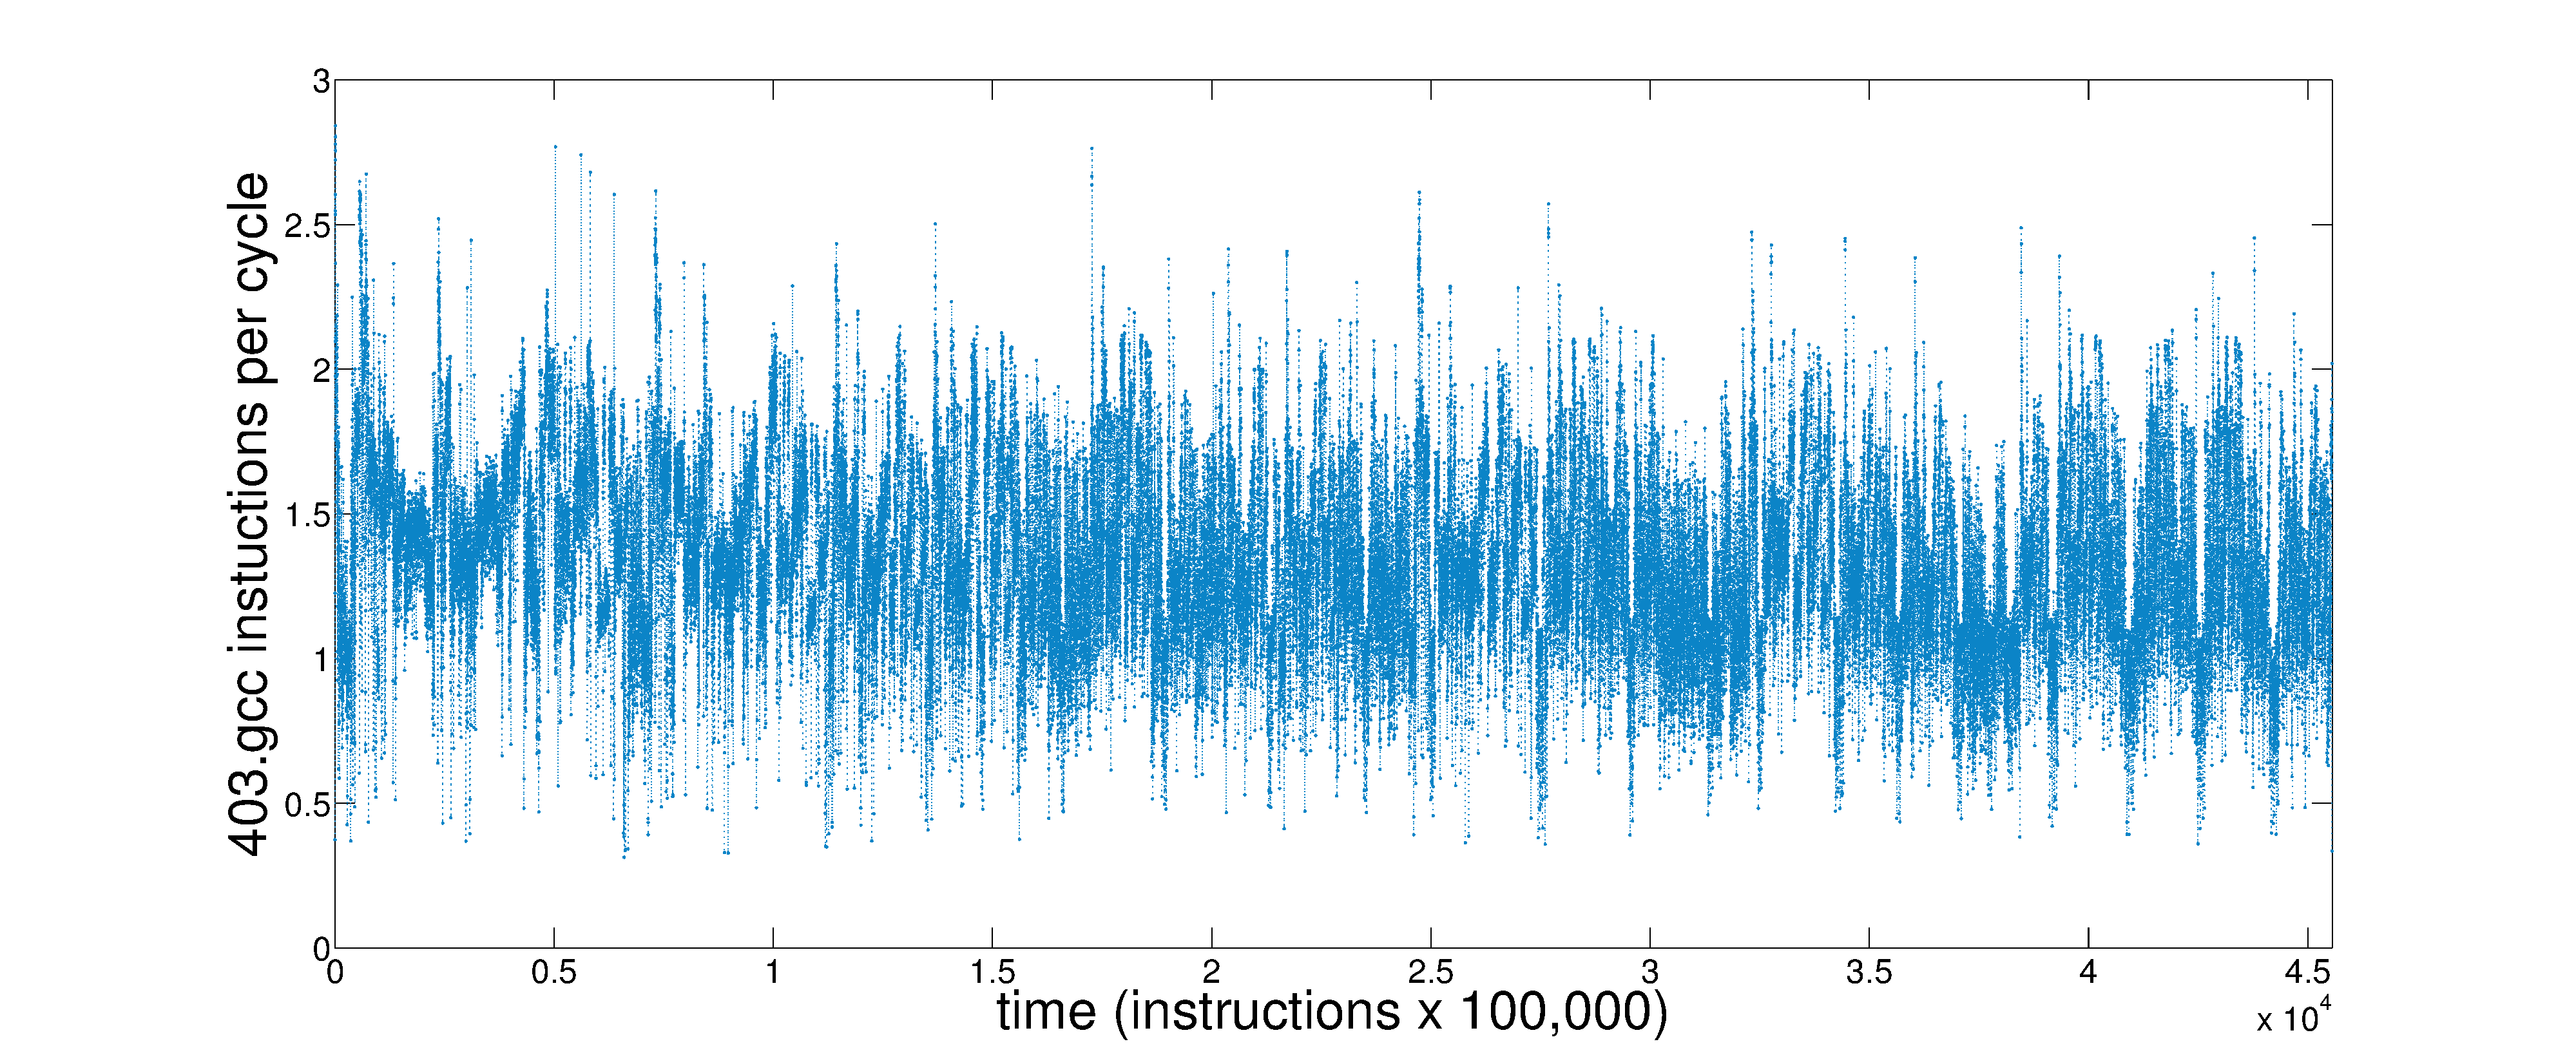
\includegraphics[width=\columnwidth]{figs/gccfullts}
    \caption{The instructions executed per CPU clock cycle (IPC) during the execution of \gcc. Each point is the average IPC during a 100,000 instruction period.}
    \label{fig:gcc-ts}
  \end{figure}

\subsubsection{\svd {\color{blue} EDITABLE}}

\svd is a Fortran program from the LAPACK suite \cite{lapack} which calculates the singular value decomposition (SVD) of a rectangular $M$ by $N$  real-valued matrix which need not contain special structure such as symmetric, positive definite etc. To execute this program we input a 750 x 1000 matrix of randomly generated entries\footnote{Multiple randomly generated matrices were investigated but no measurable effect was present in the resulting time series.}. A ``regime-colored" time series of the IPC of this program is shown in Figure \ref{fig:svd-ts-colored}. We now describe why this is done.

\begin{figure}[t]
    \centering
    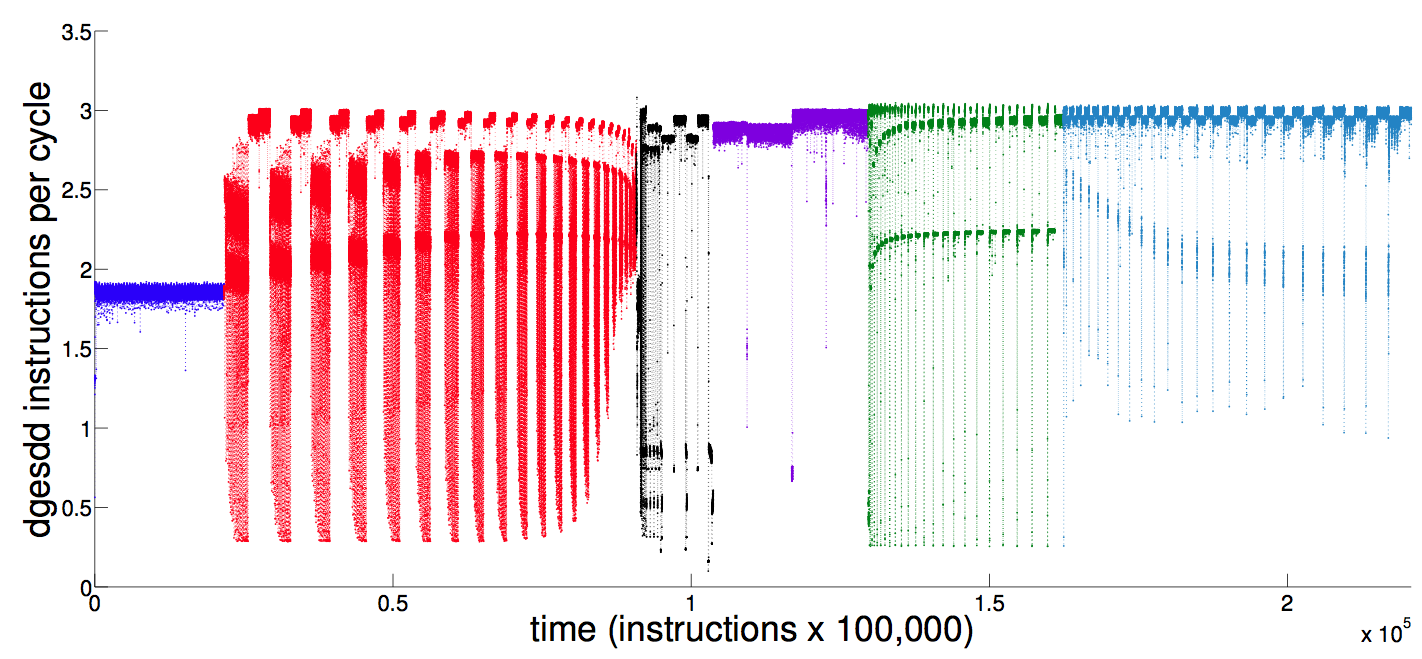
\includegraphics[width=\columnwidth]{figs/SVD1RegimesColored}
    \caption{The instructions executed per CPU clock cycle (IPC) during the execution of \svd. Each point is the average IPC during a 100,000 instruction period. The colors correspond to the six different regimes detected visually.}
    \label{fig:svd-ts-colored}
  \end{figure}

\svd brings up a very interesting point: as we observe a system the generating process can change in complexity over time. While it is clear in Figures \ref{fig:col-ts} and \ref{fig:gcc-ts} that a single system is being observed, it also appears \emph{visually} that the complexity of these two time series is consistent over time, i.e., while they are both complicated they don't appear to increase or decrease in complexity over the range of the program. \svd (seen in Figure \ref{fig:svd-ts-colored}) is different however, at least visually. Like Figures \ref{fig:col-ts} and \ref{fig:gcc-ts}, Figure \ref{fig:svd-ts-colored} is a single time series of the IPC of \svd, however as time progresses it is clear that something drastically changes in the underlying generating process and the structure of the time series  \emph{visually} switches between ``regimes".\footnote{It should be noted that a windowed version of the complexity metric we discuss in Section~\ref{sec:meaComplex} has been used to detect siezures in brainwave data \cite{cao2004det}, which can be viewed as regime detection. When we used this method on \svd the regimes we chose visually had different entropies from regime to regime but but the regime boundaries seem fractal in nature. This is something we plan to investigate in future work. For the purposes of this paper the regime detection was done visually.}

This is caused by the code of \svd moving between different subroutines as the SVD algorithm evolves, something not present in either \gcc or \col. We call these changes in \svd dynamics \emph{\svd regimes} and we have colored each of the six regimes differently in Figure \ref{fig:svd-ts-colored}. The advantage to splitting \svd into these regimes is to explore how complexity and predictability evolve over time for a system in drift.  Note, the purpose of this paper is \emph{not} to rigorously explore regime detection but to explore quantifying complexity of a time series. As such, making these regime splits serves to provide an additional 90 unique time series\footnote{Six Regimes with 15 individual runs each.} to explore. For notational convenience we refer to these time series as {\tt dgesdd$_i$} with $i \in \{1\dots6\}$ where $i$ corresponds to a regime of \svd, ordered from left to right.


For regimes \cite{cao2004det}
